\chapter{Heurísticos}
\label{cap:heuristicos}
Este capítulo presenta los conceptos de heurístico y evaluador heurístico.
Define la función de evaluación heurística que deben implementar los evaluadores heurísticos que necesitan las estrategias presentadas en el capítulo~\ref{cap:estrategias}.
Se describen dos evaluadores heurísticos que implementan la función de evaluación de forma genérica, mediante tablas de valores y redes neuronales; y se estudiará una forma de entrenarlos con aprendizaje con refuerzo mediante el método de las diferencias temporales.
Estos evaluadores serán en la medida de lo posible, independientes del juego pues no necesitarán información sobre el mismo.
Por último, se presentarán también los evaluadores heurísticos desarrollados específicamente para los juegos del Conecta-4 y del Go.

\bigskip
Un \textbf{heurístico} es una función o algoritmo que nos ayuda a encontrar soluciones ``buenas'' a los problemas.
El heurístico proporciona información que nos permite decidir entre varias alternativas, aunque esta información puede estar incompleta o no ser completamente fiable.
Los heurísticos generalmente se emplean en problemas donde no se puede obtener una solución óptima bajo los requisitos dados de tiempo y espacio. En esos casos nos conformamos con una buena solución.

%En esta sección se describen los evaluadores heurísticos genéricos que emplean los agentes.
%Con genérico queremos decir que son independientes del tipo de juego.
%Los heurísticos genéricos serán aquellos que necesiten de un entrenamiento previo; pues no usan información alguna del dominio.
%Por ello también se estudiará el aprendizaje con refuerzo mediante el método de las diferencias temporales, lo que nos permitirá entrenar a los dos evaluadores heurísticos propuestos: la tabla de valo y la red neuronal.
%Comenzaremos definiendo qué es un heurístico y un evaluador heurístico.

Un \textbf{evaluador heurístico} nos permite evaluar si una situación dada nos es favorable o no, usando para ello una función de evaluación heurística.
El agente presentado en \ref{ssec:evaluador_heuristico} al que llamábamos, valga la redundancia, \textit{Agente evaluador heurístico}, usa un evaluador heurístico para decidir el próximo movimiento.

\bigskip
A continuación se define la función de evaluación heurística, cómo implementar esta función dependerá de cada juego; aunque también se puede implementar de manera genérica para cualquier juego como se verá en las siguientes secciones.

\section{Función de evaluación heurística}
\label{sec:funcion_evaluacion_heuristica}
Este apartado describe las características que deben cumplir las funciones de evaluación heurísticas, de forma que permitan a la estrategia que las use cumplir su objetivo.

\bigskip
Una función de evaluación devuelve una estimación de la utilidad esperada de una posición dada del juego, independientemente de si se trata de una posición final o no.
Por un lado, la función de evaluación debería ordenar los estados terminales del mismo modo que la función de utilidad verdadera del juego.
Por otro lado, para estados no terminales la función de evaluación debería estar fuertemente correlacionada con las posibilidades reales de ganar.
En último lugar, el cálculo no debe emplear demasiado tiempo, ya que la función será invocada repetidas veces por la estrategia para decidir un único movimiento.

La función de evaluación heurística empleada para evaluar los estados de un juego debe devolver un valor positivo si el estado es favorable para nuestro jugador (que llamaremos \textit{MAX} siguiendo la terminología de minimax introducida en \ref{ssec:minimax}), un valor negativo si el estado es desfavorable y cero si el estado es indiferente (no es favorable ni desfavorable).
Este valor será más grande cuanto más favorable sea el estado para \textit{MAX} y más pequeño cuanto más desfavorable sea.
Llamaremos a la función de evaluación \textit{e(n)}, donde \textit{n} es el estado a evaluar:
\begin{equation}
e(n) = \left\{\begin{array}{ll}
\infty & \textnormal{si \textit{n} es un estado terminal y gana \textit{MAX}}\\
>0 & \textnormal{si \textit{n} es favorable para \textit{MAX}}\\
0 & \textnormal{si \textit{n} es indiferente (``empate'')}\\
<0 & \textnormal{si \textit{n} es desfavorable para \textit{MAX}}\\
-\infty & \textnormal{si \textit{n} es un estado terminal y pierde \textit{MAX}}\\
\end{array}\right. \label{eq:heuristico}
\end{equation}

Dos formas de implementar esta función de manera genérica (sin necesitar conocimiento del juego en cuestión) son las tablas de valores y las redes neuronales que darán lugar a nuestros dos evaluadores genéricos.
Para ello es necesario que dispongan de algún tipo de aprendizaje que les permita aprender cuándo un estado es favorable o no.

\bigskip
A continuación se presenta el aprendizaje con refuerzo mediante el método de las diferencias temporales, que será la forma de entrenar a los evaluadores con tablas de valor y redes neuronales.

\section{Aprendizaje con refuerzo}
\label{sec:aprendizaje_refuerzo}
El \textbf{aprendizaje con refuerzo} es un método de aprendizaje automático en el que el algoritmo aprende observando el medio que le rodea.
La información de entrada es el \textit{feedback} o retroalimentación que obtiene del medio como respuesta a sus acciones.
Por lo tanto, el sistema aprende por sí mismo a base de ensayo-error.
Un agente que use aprendizaje con refuerzo necesita saber que algo bueno ha ocurrido cuando gana y que algo malo ha ocurrido cuando pierde.
Esta clase de retroalimentación se denomina \textbf{recompensa} (\textit{reward}).

En este tipo de aprendizaje el agente no tiene ningún conocimiento a priori sobre el entorno, ya que no es necesario.
Lo único que tiene que saber el agente es cuándo ha ganado o ha perdido y puede usar esta información para aprender una función de evaluación que proporcione estimaciones certeras y razonables de la probabilidad de ganar a partir de una situación dada.

En nuestro caso no entrenaremos directamente al agente sino al evaluador heurístico que usa.
El entrenamiento se realizará mediante el método de las diferencias temporales, que se explica a continuación.

\subsection{Método de las diferencias temporales}
\label{ssec:diferencias_temporales}
Llamaremos función de recompensa a la función que indica al evaluador heurístico cuándo ha ganado, ha empatado o ha perdido; y función de utilidad a la función de evaluación que debe aprender y que proporciona la recompensa esperada a partir de una situación dada.

La función de recompensa (R) define el objetivo del problema: obtener la mayor recompensa posible.
Dado un estado, devuelve su valor de recompensa real.
Este valor puede ser por ejemplo un número positivo en caso de que el estado sea ganador, negativo y opuesto si es perdedor y cero si es empate.

La función de utilidad (U) define lo ``deseable'' que es un estado, es decir, su propio valor de recompensa más la utilidad esperada de sus estados sucesores.
Dado un estado, devuelve la recompensa esperada a largo plazo.
La acción o movimiento a elegir en cada momento es la que lleva a un estado de mayor utilidad.

El \textbf{método de las diferencias temporales} (\textit{TD}) consiste en usar las acciones realizadas para ajustar los valores de los estados correspondientes según los valores de recompensa obtenidos.
Se elaboran unas secuencias de entrenamiento, en este caso las secuencias de entrenamiento serán partidas completas de un juego; y partiendo de unos valores iniciales cualesquiera, en cada paso (estado \textit{n} $\rightarrow$ sucesor \textit{s}) de cada secuencia se actualiza el valor de utilidad correspondiente:
\begin{displaymath}
U(n) = U(n) + \alpha(R(n) + U(s) - U(n))
\end{displaymath}
donde $\alpha$ es la tasa de aprendizaje, expresada como un escalar en el intervalo $(0,1)$.
La diferencia de utilidades entre estados sucesivos es la regla de aprendizaje por diferencias temporales y los valores así calculados convergen a las utilidades óptimas de los estados.

En el caso de los juegos el valor inicial de recompensa para un estado es cero.
Por lo que si el valor de utilidad del estado sucesor es menor que el valor del padre, el valor de este último desciende; por el contrario, si el valor de utilidad del estado sucesor es mayor que el valor del padre, el valor de este último aumentará.

Para garantizar que se obtiene una buena estrategia, se pueden realizar movimientos exploratorios durante el entrenamiento.
Para ello se introduce una componente aleatoria para los movimientos del evaluador a entrenar: cada movimiento tendrá una probabilidad de ser aleatorio (exploratorio); en caso de que el movimiento sea exploratorio, no se entrenará al evaluador.

El método de las diferencias temporales se puede aplicar a cualquier juego, pues no necesita de un modelo concreto para llevar a cabo sus actualizaciones; el entorno proporciona las conexiones entre los diferentes estados en forma de movimientos posibles.
Este tipo de aprendizaje es sencillo y no requiere de mucho tiempo de cálculo, pero tiene la desventaja de que el aprendizaje el lento.

\bigskip
Las siguientes secciones describen los evaluadores que implementan la función de evaluación de forma genérica, y que son entrenados empleando aprendizaje con refuerzo mediante el método de las diferencias temporales.

\section{Tabla de Valor}
\label{sec:tabla_valor}
El primer evaluador heurístico que presentamos es la tabla de valor.
Este evaluador implementa la función de evaluación mediante una tabla que almacena el valor de utilidad para cada estado.
El evaluador es entrenado mediante el método de las diferencias temporales; actualizando los valores de la tabla en cada paso del entrenamiento:
\begin{displaymath}
tabla(n) \leftarrow tabla(n) + \alpha(tabla(s) - tabla(n))
\end{displaymath}
donde \textit{n} es el estado cuyo valor se actualiza, \textit{s} es el sucesor del estado \textit{n} elegido y $\alpha$ es la tasa de aprendizaje.

Los valores de utilidad de cada estado al final del entrenamiento se corresponden con el valor de evaluación que devolverá el evaluador para cada estado:
\begin{displaymath}
e(n) = tabla(n)
\end{displaymath}

La ventaja de este evaluador es que es independiente del juego y podrá usarse en cualquiera de los juegos propuestos.
La principal desventaja es la propia tabla de valores, debido al consumo de memoria.

\section{Red Neuronal}
\label{sec:red_neuronal}
El segundo evaluador heurístico es una red neuronal.
Este evaluador implementa la función de evaluación mediante una red neuronal multicapa con el algoritmo de aprendizaje mediante retropropagación.

Para diseñar la arquitectura de la red, se seleccionan una serie de características del entorno.
El número de neuronas de entrada dependerá de las características elegidas, es decir, de cómo se codifiquen los estados de los juegos; lo que implica que este evaluador no pueda ser del todo independiente del juego.\footnote{En \ref{ssec:redNeuronal_conecta4} y \ref{ssec:redNeuronal_go} se definen la funciones de codificación propuestas para los estados del juego del Conecta-4 y del Go.}

La red tiene dos neuronas de salida para realizar la evaluación.
La primera ($p_1$) se interpreta como la probabilidad de que la posición sea ganadora para el primer jugador; y la segunda ($p_2$) como la probabilidad de que la posición sea ganadora para el segundo jugador.
El resultado de la evaluación es la diferencia entre las dos salidas:
\begin{displaymath}
e(n) = p_1 - p_2
\end{displaymath}
donde \textit{n} es el estado evaluado.

La red cuenta con una sola capa intermedia de neuronas.
El número de neuronas de esta capa será un parámetro adicional de la red.
La función que cumple dicha capa intermedia es tratar de realizar una proyección en la que resulten separables linealmente los patrones de entrada de manera que las unidades de salida pueda realizar una clasificación correcta.
Establecer de antemano el número de neuronas intermedias no es sencillo y puede ser necesario realizar varios experimentos antes de encontrar la estructura ideal de la red para un determinado juego.

La forma de entrenar una red neuronal multicapa mediante aprendizaje por refuerzo es un algoritmo conocido como $TD(\lambda)$ (nosotros usaremos la versión simplificada del método TD, visto en el apartado~\ref{ssec:diferencias_temporales}); entrenando la red del siguiente modo: cuando una posición del juego es final, se entrena con la salida correcta (posición ganadora, perdedora o de empate para el jugador); cuando la posición no sea final, se entrena la red para que su evaluación sea parecida a la de la siguiente posición en la secuencia de entrenamiento.

La red dispone también de dos parámetros adicionales para tener un mayor control sobre su aprendizaje.
Por un lado tiene una \textit{tasa de aprendizaje} que permite ajustar la velocidad a la que aprende la red.
Por otro lado tiene un \textit{momento} de entrenamiento que indica la influencia que tendrá la iteración anterior sobre la actual.
Ambos valores son porcentajes expresados mediante escalares en el intervalo $[0,1]$.

%Puede ser necesario un cierto grado de experimentación antes de dar con un red correctamente entrenada.
%Además, pueden presentarse oscilaciones en el aprendizaje de la red.

\section{Heurísticos para el Conecta-4}
\label{sec:heuristicos_conecta4}
En esta sección se define una función heurística que proporciona una evaluación de los estados del juego para el Conecta-4, empleando para ello una matriz de posibilidades.
También se presenta una función de codificación de los estados del juego para un evaluador con red neuronal.

\subsection{Matriz de posibilidades}
\label{ssec:matriz_posibilidades}
Dado un estado del juego la función de evaluación heurística debe devolver un número positivo si el estado es favorable para nuestro jugador, un número negativo si el estado es desfavorable y cero si es indiferente.

Llamaremos a nuestro jugador \textit{MAX} y a su oponente \textit{MIN}.
La función de evaluación para los estados del juego Conecta-4 se define como:
\emph{número de posibilidades de conectar 4 fichas que tiene \textit{MAX}, menos el número de posibilidades de conectar 4 fichas que tiene \textit{MIN}.}

Para determinar el número de posibilidades de conectar 4 fichas se emplea una \textit{matriz de posibilidades}.
A continuación se detalla un método para construir la matriz de posibilidades.
Por simplicidad y sin perder genericidad se considera una versión simplificada del juego: el Conecta-3 sobre un tablero 4x4.

Cada posición del tablero tiene un número de posibilidades distintas de conectar 3 fichas.
La figura~\ref{fig:conecta3_posibilidades1} muestra las posibilidades de conectar 3 fichas que tiene la posición correspondiente a la esquina inferior izquierda del tablero.
Esta posición interviene en tres posibilidades que numeramos del 0 al 2.
La figura~\ref{fig:conecta3_posibilidades2} muestra las posibilidades de conectar 3 fichas que tiene la posición siguiente.
En este caso también tiene tres posibilidades que numeramos del 3 al 5.
\begin{figure}[h]
	\centering
	% Primera imagen
	\begin{minipage}[t]{0.3\linewidth}
		\centering
		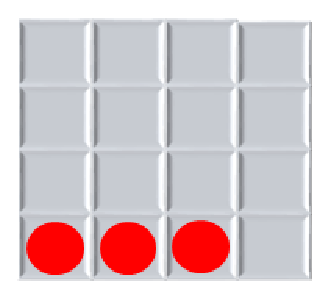
\includegraphics[scale=0.5]{contenido/cap4/imagenes/posibilidadesConecta3_01.eps}
	\end{minipage}
	%\hspace{0.5cm}
	% Segunda imagen
	\begin{minipage}[t]{0.3\linewidth}
		\centering
		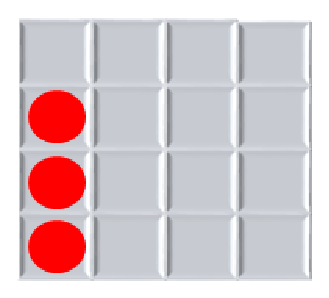
\includegraphics[scale=0.5]{contenido/cap4/imagenes/posibilidadesConecta3_03.eps}
	\end{minipage}
	%\hspace{0.5cm}
	% Tercera imagen
	\begin{minipage}[t]{0.3\linewidth}
		\centering
		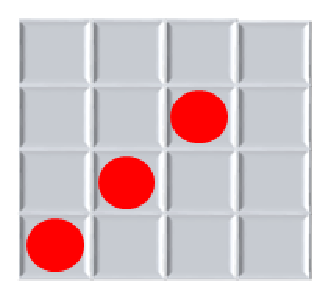
\includegraphics[scale=0.5]{contenido/cap4/imagenes/posibilidadesConecta3_02.eps}
	\end{minipage}
	\caption[Posibilidades en el Conecta-3 (I)]{Posibilidades 0, 1 y 2.}
	\label{fig:conecta3_posibilidades1}
\end{figure}

\begin{figure}[h]
	\centering
	% Primera imagen
	\begin{minipage}[t]{0.3\linewidth}
		\centering
		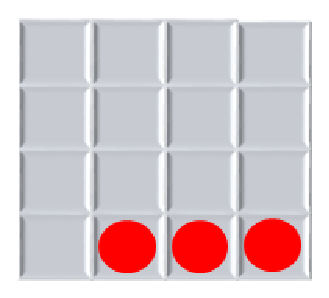
\includegraphics[scale=0.5]{contenido/cap4/imagenes/posibilidadesConecta3_01b.eps}
	\end{minipage}
	%\hspace{0.5cm}
	% Segunda imagen
	\begin{minipage}[t]{0.3\linewidth}
		\centering
		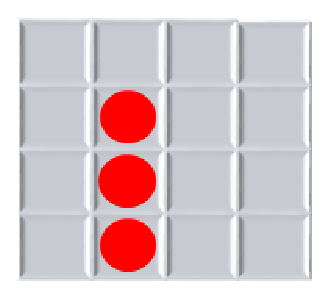
\includegraphics[scale=0.5]{contenido/cap4/imagenes/posibilidadesConecta3_03b.eps}
	\end{minipage}
	%\hspace{0.5cm}
	% Tercera imagen
	\begin{minipage}[t]{0.3\linewidth}
		\centering
		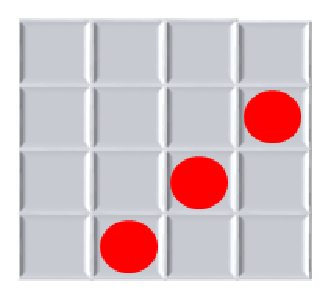
\includegraphics[scale=0.5]{contenido/cap4/imagenes/posibilidadesConecta3_02b.eps}
	\end{minipage}
	\caption[Posibilidades en el Conecta-3 (II)]{Posibilidades 3, 4 y 5.}
	\label{fig:conecta3_posibilidades2}
\end{figure}

Recorriendo todas las posiciones del tablero y enumerando todas las posibilidades en las que interviene cada posición del tablero se obtiene una matriz de posibilidades como la mostrada en la figura~\ref{fig:conecta3_matrizPosibilidades}.

\begin{figure}[h]
	\centering
	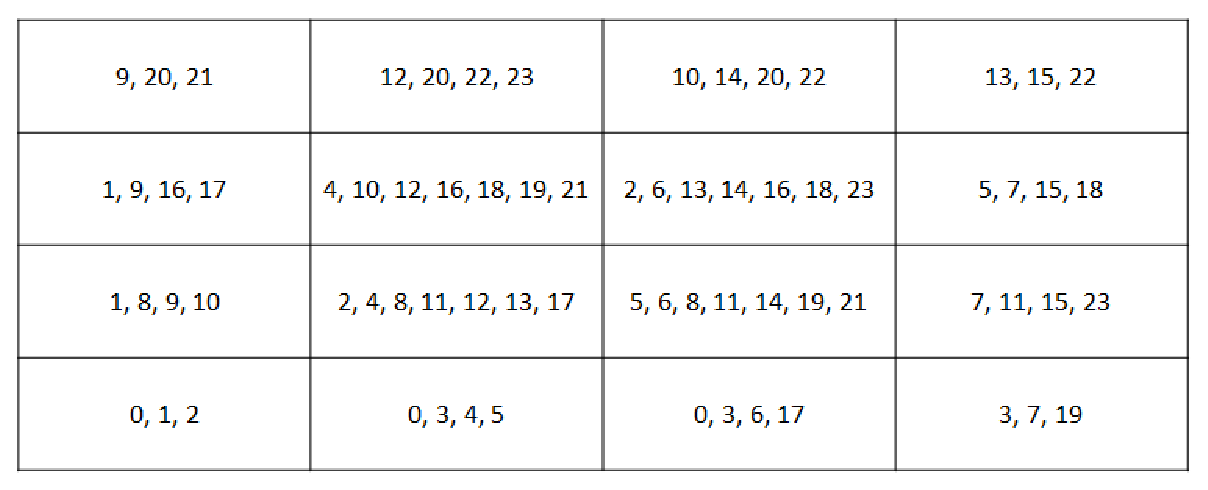
\includegraphics[scale=0.6]{contenido/cap4/imagenes/matrizPosibilidades_Conecta3.eps}
	\caption{Matriz de posibilidades.}
	\label{fig:conecta3_matrizPosibilidades}
\end{figure}

Existen 24 posibilidades de conectar 3 fichas.
Las posiciones menos interesantes del tablero corresponden a las cuatro esquinas.
Las posiciones situadas en las columnas centrales, por el contrario, son las que ofrecen más posibilidades.

Para realizar la evaluación, la función heurística tiene acceso a la matriz de posibilidades del tablero.
Cada jugador dispone de un vector de longitud \textit{n}, donde\textit{ n} es el número de posibilidades de conectar \textit{k} fichas en el tablero.
Para cada casilla ocupada en el tablero se actualizan los vectores adecuadamente con la ayuda de la matriz de posibilidades: si una casilla está ocupada por una ficha de \textit{MAX}, se elimina del vector de \textit{MIN} todas las posibilidades en las que interviene; y si está ocupada por una ficha de \textit{MIN}, se elimina las posibilidades del vector de \textit{MAX}.
El valor devuelto por la función heurística es la diferencia entre la suma de posibilidades libres en el vector de \textit{MAX} y la suma de posibilidades libres en el vector de \textit{MIN}:
\begin{displaymath}
e(n) = posibilidades_{MAX}(n) - posibilidades_{MIN}(n)
\end{displaymath}

\bigskip
A continuación se presenta el evaluador con red neuronal para el Conecta-4, definiendo la función para codificar los estados como entrada a la red.

\subsection{Red neuronal para el Conecta-4}
\label{ssec:redNeuronal_conecta4}
El evaluador con red neuronal presentado en la sección~\ref{sec:red_neuronal} necesitaba de una función de codificación de los estados de los juegos para usarlos como entrada de la red neuronal.

Para los estados del juego del Conecta-4 se codificará cada posición del tablero mediante dos entradas a la red neuronal:
\begin{itemize}
\renewcommand{\labelitemi}{-}
	\item La primera entrada será 1 si hay una ficha del primer jugador y 0 en caso contrario.
	\item La segunda entrada será 1 si hay una ficha del segundo jugador y 0 en caso contrario.
\end{itemize}
De este modo, para un tablero \textit{nxm} se necesitan \textit{2xnxm} entradas en la red neuronal.

El número de neuronas de la capa intermedia no está fijado; lo que permite realizar varias pruebas con diferentes valores hasta encontrar el valor que mejor resultados obtenga.

\bigskip
Una vez definidos los heurísticos específicos para el juego del Conecta-4, presentamos los heurísticos para el juego del Go.

\section{Heurísticos para el Go}
\label{sec:heuristicos_go}
En esta sección se estudiarán varios heurísticos para el juego del Go que permitan decidir si un estado del juego es mejor que otro.

\bigskip
%En la actualidad los computadores juegan al Go a nivel aficionado, debido a que el factor de ramificación para un tablero 19x19 es muy elevado (comenzando en 361).
%Este proyecto estudia una versión reducida en un tablero de 9x9;
%aunque los heurísticos aquí descritos son válidos para cualquier dimensión del tablero.

Las funciones heurísticas están basadas en el objetivo principal del juego: controlar el mayor número de territorios del tablero, entendiendo por territorios el número de intersecciones libres conquistadas por un jugador.
Ubicar piedras juntas ayuda a protegerlas entre sí y evitar ser capturadas. 
Por otro lado, colocar piedras de forma separada hace que se tenga influencia sobre una mayor porción del tablero. 
Parte de la dificultad estratégica del juego surge a la hora de encontrar un equilibrio entre estas dos alternativas. 
Los jugadores pueden jugar tanto de manera ofensiva como defensiva y deben elegir entre tácticas de urgencia y planes a largo plazo más estratégicos.

Teniendo esto en cuenta se definen tres evaluadores heurísticos: uno basado únicamente en los territorios conquistados por cada jugador, y los otros dos en función de los puntos conseguidos por cada jugador hasta el momento, según las reglas de puntuación japonesas para el primer evaluador y según las reglas chinas para el segundo evaluador.

\subsection{Evaluador de territorios}
\label{ssec:evaluador_territorios}
El primer evaluador tiene en cuenta solamente los territorios conquistados por cada jugador.
El valor devuelto por la función heurística para un estado \textit{n} es la diferencia entre el número de territorios pertenecientes a \textit{MAX} y el número de territorios de \textit{MIN}:
\begin{displaymath}
e(n) = territorios_{MAX}(n) - territorios_{MIN}(n)
\end{displaymath}

\subsection{Evaluador de puntos JP}
\label{ssec:evaluador_puntosJP}
El segundo evaluador se basa en la puntuación de cada jugador en el estado actual, según las reglas de puntuación japonesas.
Recordemos que los japoneses cuentan un punto por cada intersección vacía dentro del territorio conquistado menos un punto por cada piedra que haya capturado el enemigo.
El valor de la función heurística para un estado \textit{n} es la diferencia entre los puntos de \textit{MAX} y de \textit{MIN} según las reglas de puntuación japonesas:
\begin{displaymath}
e(n) = puntos_{MAX}^{JP}(n) - puntos_{MIN}^{JP}(n)
\end{displaymath}

\subsection{Evaluador de puntos CH}
\label{ssec:evaluador_puntosCH}
El último evaluador propuesto es igual que el anterior pero teniendo en cuenta las reglas de puntuación chinas.
Los jugadores chinos cuentan un punto por cada intersección vacía dentro del territorio más un punto por cada ficha del jugador sobre el tablero.
Para un estado \textit{n}, el valor de la función heurística es la diferencia de puntos entre \textit{MAX} y \textit{MIN} según las reglas de puntuación chinas:
\begin{displaymath}
e(n) = puntos_{MAX}^{CH}(n) - puntos_{MIN}^{CH}(n)
\end{displaymath}

\bigskip
La siguiente sección presenta el evaluador con red neuronal para el Go, definiendo la función para codificar los estados como entrada a la red.

\subsection{Red neuronal para el Go}
\label{ssec:redNeuronal_go}
Se define a continuación la función de codificación para los estados del Go que necesita la red neuronal como entrada.
El evaluador con red neuronal se presentó en la sección~\ref{sec:red_neuronal} de manera general.

\bigskip
La forma de codificar los estados será la misma que la empleada en el juego del Conecta-4.
Cada posición del tablero se codifica mediante dos entradas a la red neuronal:
\begin{itemize}
\renewcommand{\labelitemi}{-}
	\item La primera entrada será 1 si hay una ficha del primer jugador y 0 en caso contrario.
	\item La segunda entrada será 1 si hay una ficha del segundo jugador y 0 en caso contrario.
\end{itemize}
Para un tablero de \textit{nxn} se necesitan \textit{2xnxn} entradas en la red neuronal.

El número de neuronas de la capa intermedia tampoco está fijado para la red neuronal del Go porque puede ser útil modificar este número en función del tamaño del tablero de juego para encontrar la red neuronal ideal que juegue al Go.
